\chapter{Overview of techniques}
This chapter will introduce the techniques used to simulate the destructible environment. First, it will talk about the development of the destructible environment in a few games and game engines and then about general approaches to this problem. In this chapter, we will use word object as a reference to buildings, crates, doors, etc., excluding terrain, skyboxes and characters.

\section{Game engine approaches}
\begin{itemize}
\item \textbf{Object replacement or removal} was the first method used to simulate the destructible environment in a computer game. Mostly because it's simple and undemanding. In spite of its simplicity, it can still produce a very desirable result. In fact, it is still most widely used approach to the destructible environment in computer games.

The first 2D games featuring destructible environment are arcade games like the \emph{Space Invaders (1978)} \footnote{https://en.wikipedia.org/wiki/Space\_Invaders} where the environment is represented by cells in a grid. After taking damage, the texture of the cell is replaced by another one and the finally completely removed. The next environment destruction technique in 2D games came with games like \emph{Scorched Earth (1991)} \footnote{https://en.wikipedia.org/wiki/Scorched\_Earth\_(video\_game)} and \emph{Worms (1995)} \footnote{https://www.team17.com/games/worms-original}. Collision and removal of terrain in those games is based on individual pixels which creates more realistic visual effect.

The most common implementation of destructible objects in 3D games has not changed much over the years. Every object that the player is able to modify has a set of other models prepared. Based on how much damage is applied, the models are swapped and eventually removed completely \ref{doors}. To make the removal look natural it is usually accompanied by animations, debris and dust generation. The downfall of this method is the necessity to replace the whole in-game object. In order to make the game look realistic, there has to be a large number of objects pre-made for different scenarios and it has little flexibility to react to specific player actions. As an example, in the \emph{Source} engine, you can see that the hole in the doors \ref{doors} is always in the same place without considering the point of impact.


\begin{figure}[ht!]
\label{doors}
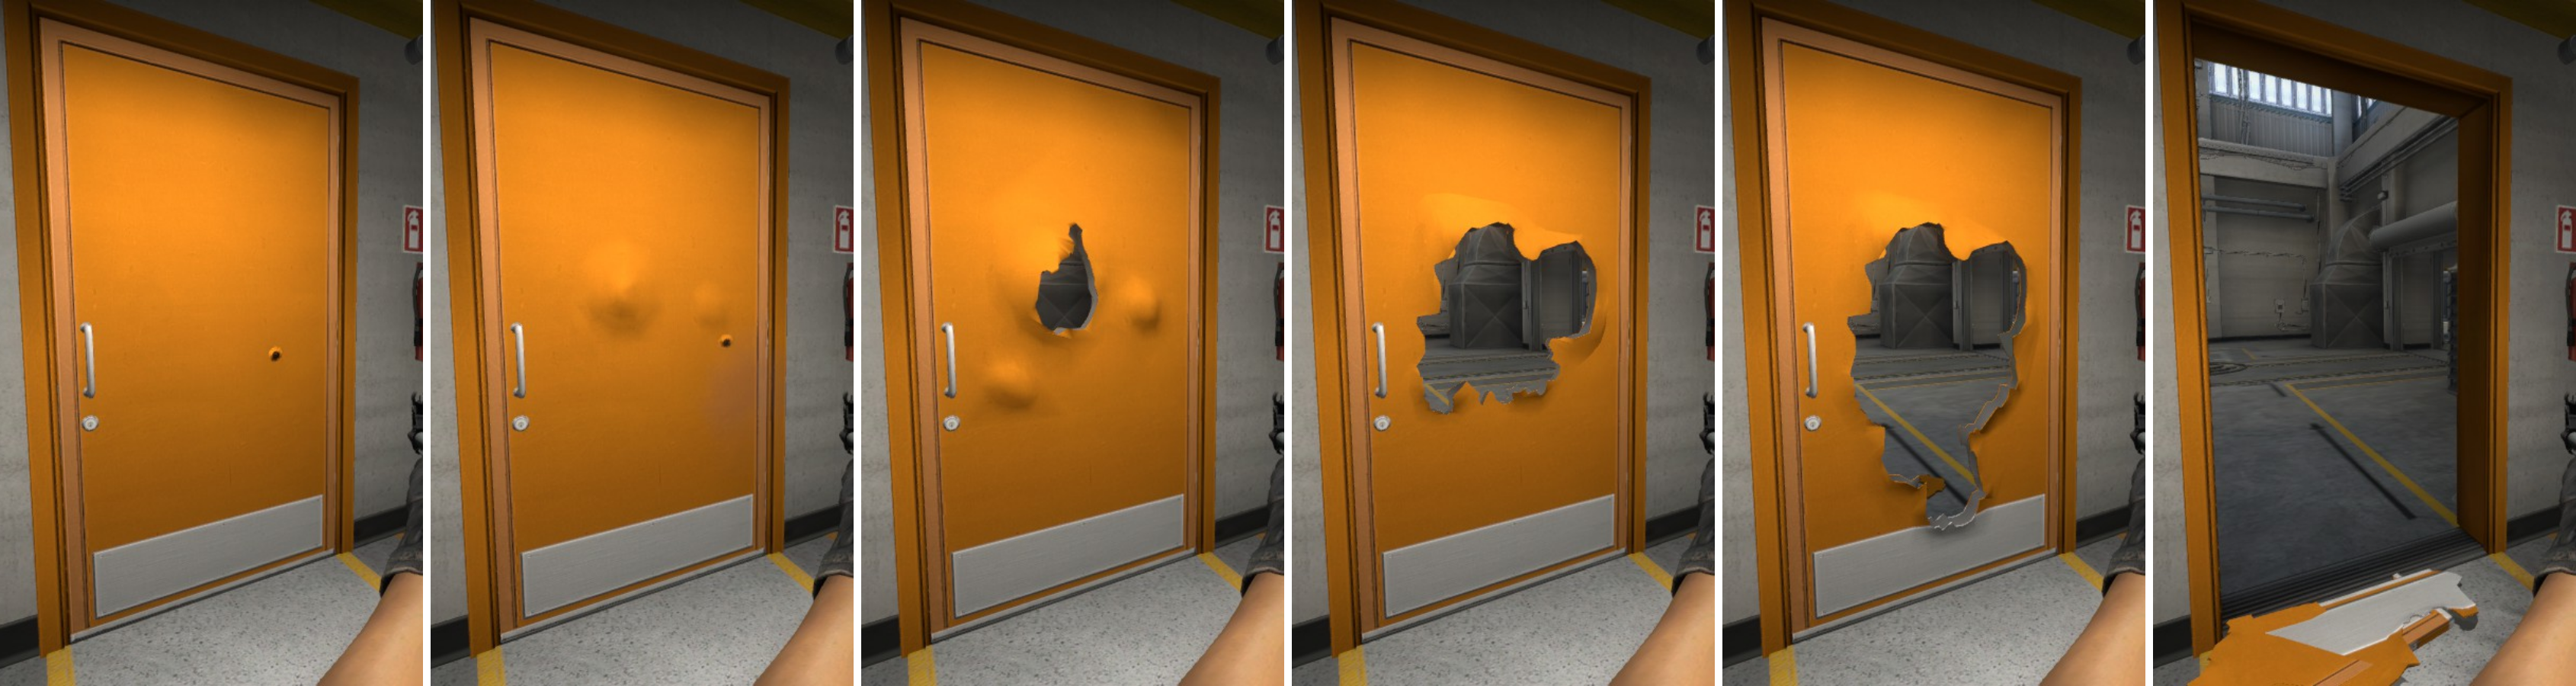
\includegraphics[width=\textwidth]{img/doors}
\caption{Source engine swapping door models}
\end{figure}

\item \textbf{\emph{Geo-Mod}} \cite{geomod} or \emph{Geometry Modification Technology} is an engine developed for the \emph{Red Faction (2001)} \footnote{http://redfaction.wikia.com/wiki/Red\_Faction} video game. It allows players to modify and make holes in the terrain using the solution of creating objects representing an empty space. Even though the engine doesn't work well with the buildings and other objects, it represents one of the first major attempts to create the fully destructible 3D environment in real time constraints.


\item \textbf{\emph{Geo-Mod 2}} \cite{geomod}\footnote{Geo-Mod 2.0 presentation video https://www.youtube.com/watch?v=lICurOVsNv0} does not feature destructible terrain, instead, it uses physics simulation on specially prepared objects. A set of smaller objects is used as a ragdoll for the stress-based simulation model. This limits the engine in the scale of the game world and mutual proximity of destructible objects.


\item \textbf{\emph{Frostbite}} \footnote{http://www.frostbite.com/about/frostbite-3} engine and mainly it's component \emph{Destruction} \cite{destruction} is currently featured in the most titles featuring destructible environment. It supports the dynamic micro-destruction on the surface and the large scale predetermined destruction on whole buildings. The buildings are created from smaller parts linked together. Each part can disappear on its own and when there is not much left the whole building collapses. It doesn't use inner body stress or  any physics while doing this simulation.

\end{itemize}

\section{Soft body dynamics}

\begin{itemize}

\item \textbf{Finite Element Method} (FEM) is a means to simulate the behavior of complex objects and systems.  It uses a large number of finite volumes(cells), interconnected or not, to simulate the reaction of material to inner and outside forces. Each cell computes it's own physics states like stress or temperature and propagates the results to neighboring cells. This allows for simulation of fluid dynamics, brittle fractures \cite{brittlefracture}, ductility \cite{ductilefracture}, elasticity, heat transfer and other physical properties. It is very useful in engineering and in modeling and rendering scenes for computer generated images but FEM requires a lot of computational resources and therefore until recently it wasn't possible to implement it in real-time environment of the computer game. Now with better hardware and optimized algorithms especially developed for real-time animation, like the one O'Brien \cite{femingames} describes this method is making its way into modern games.

\item \textbf{Material Point method} (MPM) is used to simulate behavior of continuum materials. MPM is a meshfree and Arbitrary Lagrangian–Eulerian numerical method \cite{ALE}. The Lagrangian element, or a material point, is  primary representation with position, velocity and deformation gradient. Here is the simplified overview of algorithm step, for more details see Jiangs thesis\cite{jiang2015material} 
\begin{enumerate}
	\item Grid data are reinitialized to default values.
    \item Weights and weight gradients are computed on every particle.
    \item Mass and momentum are transferred from the particles to the grid.
    \item The explicit forces on nodes are computed
    \item The explicit nodal velocity update is performed
    \item Grid based collision is performed on vertices.
    \item Particles are updated from grid velocities.
\end{enumerate}
MPM is useful for both fluid and soft body dynamics. It can simulate deformation, fractures, heat transfer, melting, etc.

\begin{figure}[h!]
\label{mpm}
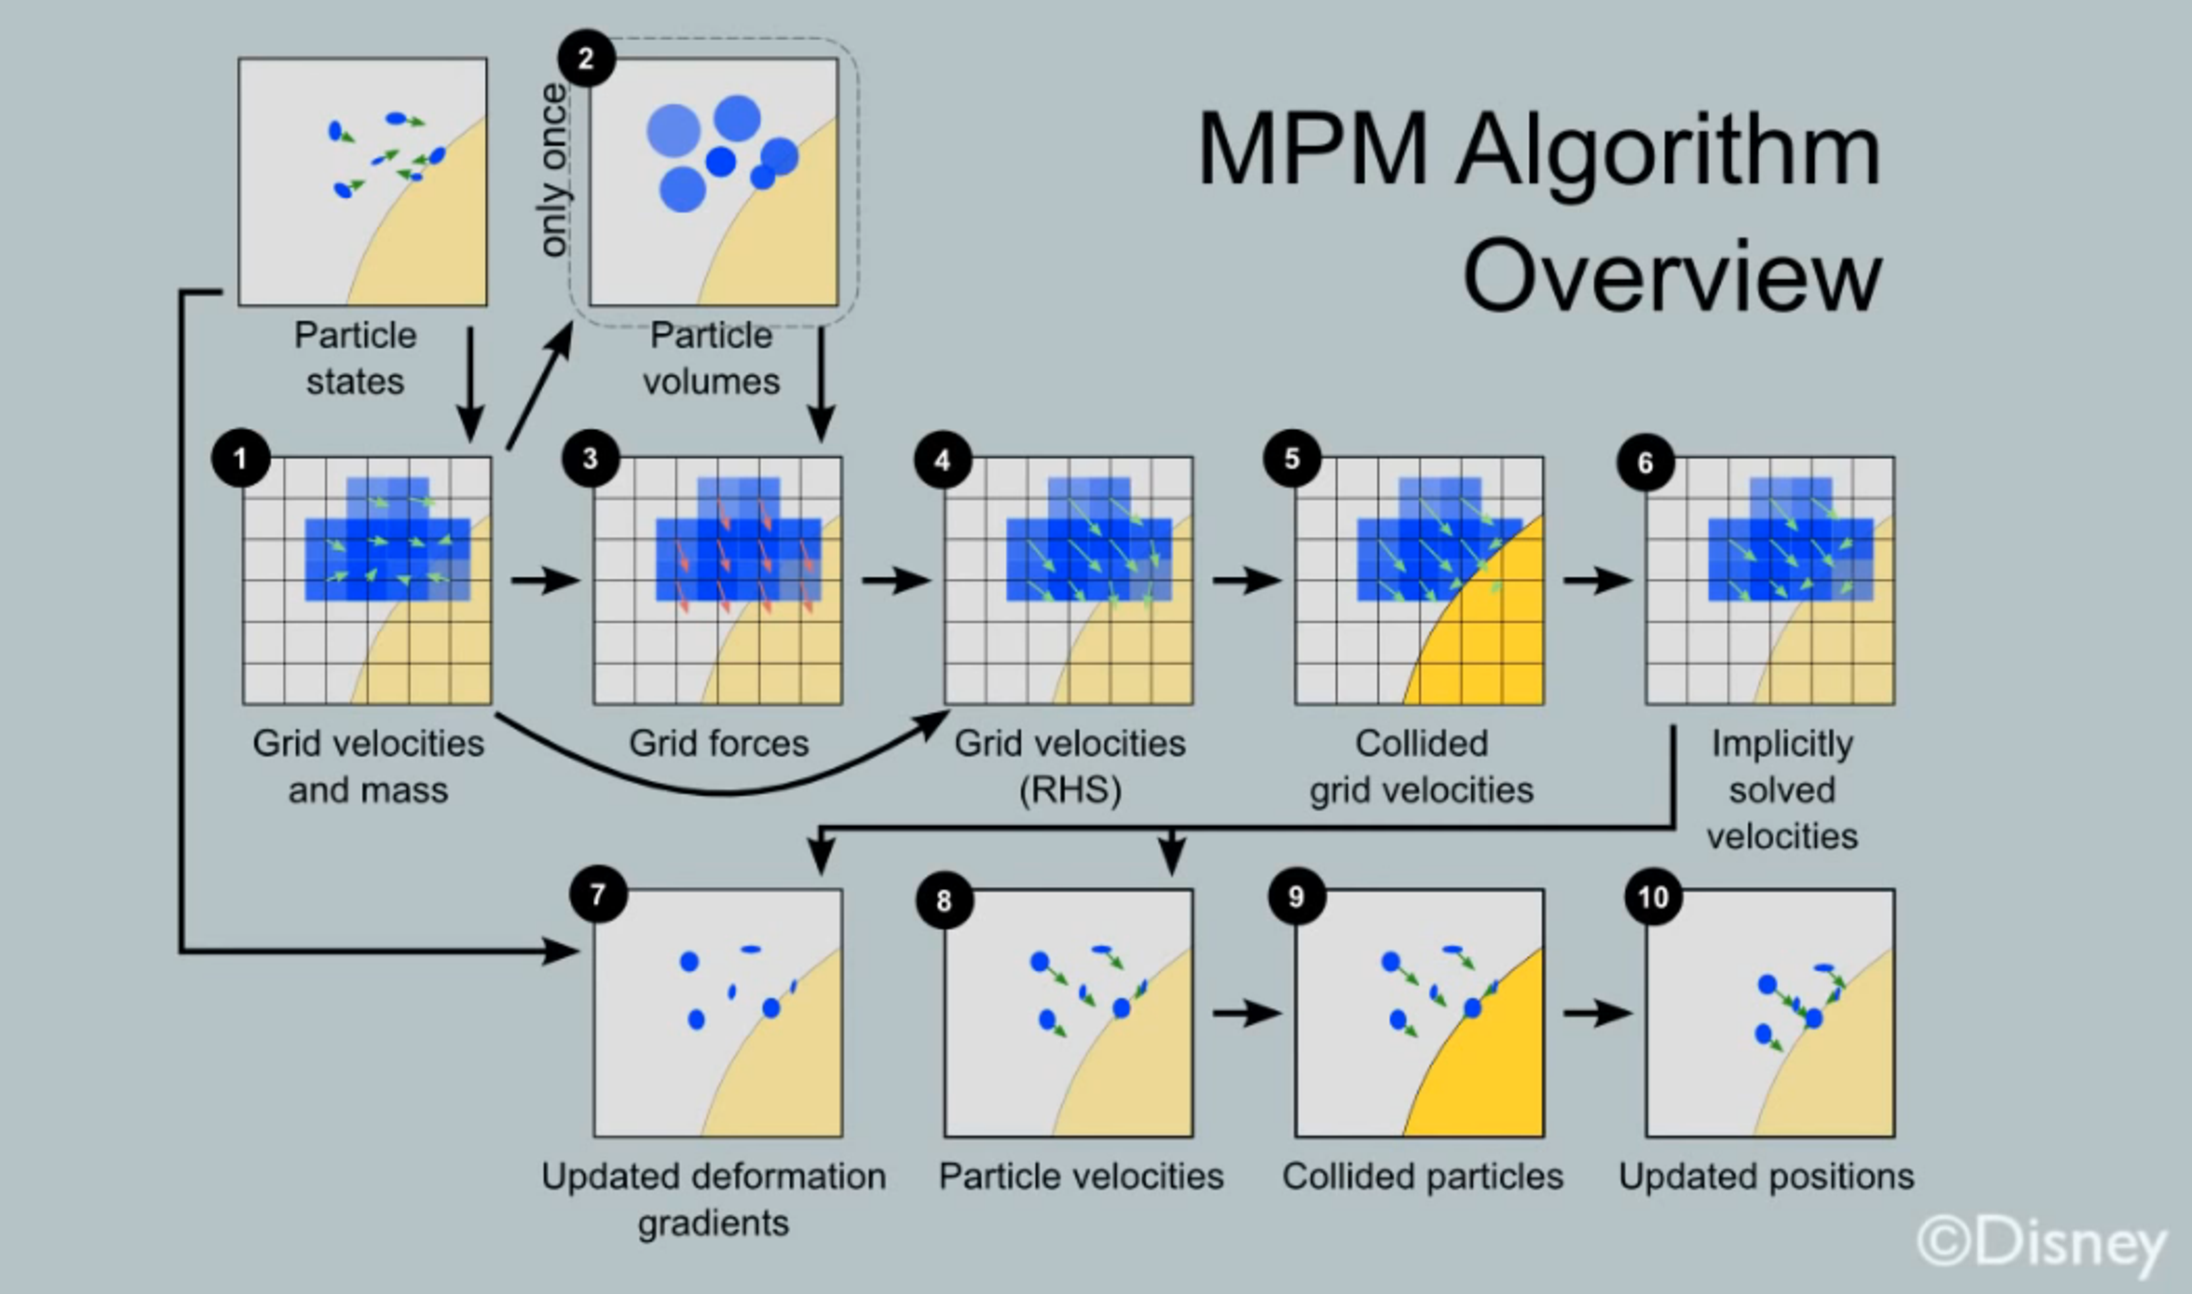
\includegraphics[width=\textwidth]{img/MPM}
\caption{MPM algorithm overview}
\end{figure}

\section{Rigid body}

\item \textbf{Voronoi tessellation} is a method of decomposing an object into a smaller parts. It can also be used for terrain generation but we will focus on object decomposition. There are simpler solutions for decomposition, for example slicing by planes or tetrahedralization, but voronoi cells look more natural. The tessellation can be done in following three steps, assuming the input is a closed triangular mesh with non-empty volume.
\begin{enumerate}
	\item Delaunay tetrahedralization \\ given points P in general position (the vertices of input mesh and a set of points inside its volume), tetrahedral mesh DT(P) can be generated satisfying following condition: no point in P is inside the circumsphere of any tetrahedra in DT(P).
    \item Creating Voronoi diagram \\ for Delaunay tetrahedralization, its dual graph (with vertices in the center of tetrahedron circumsphere) is Voronoi diagram
    \begin{figure}[h!]
		\label{DT}
        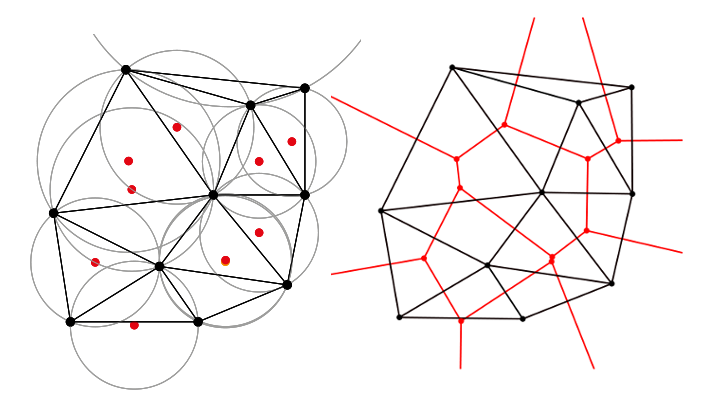
\includegraphics[width=\textwidth]{img/voro}
		\caption{Tranformation of 2D Delaunay triangularization to Voronoi diagram}
	\end{figure}
    \item Clipping Voronoi diagram
    
\end{enumerate}

clipped \cite{yan2010efficient}

\item \textbf{Precomputed fractures} TODO

\end{itemize}



